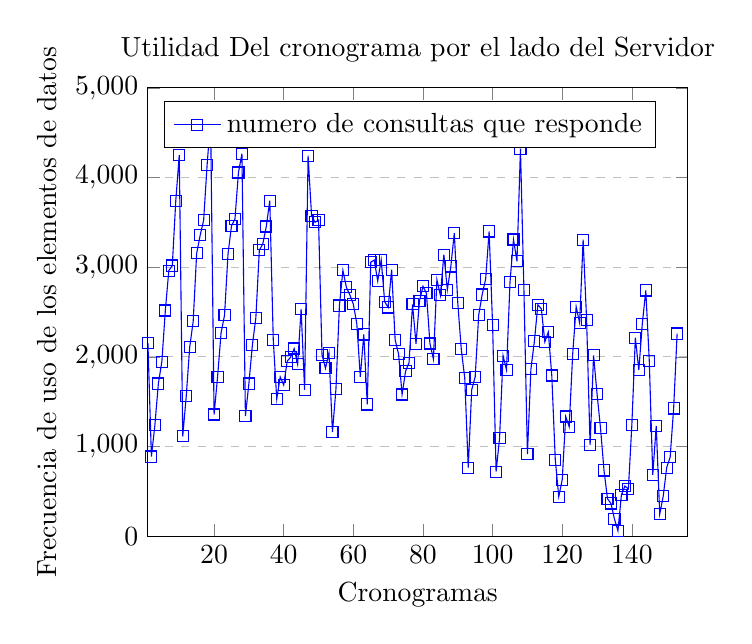
\begin{tikzpicture}
\begin{axis}[
    title={Utilidad Del cronograma por el lado del Servidor},
    xlabel={Cronogramas},
    ylabel={Frecuencia de uso de los elementos de datos},
    xmin=1, xmax=156,
    ymin=0, ymax=5000,
    xtick={},
    ytick={},
    legend pos=north west,
    ymajorgrids=true,
    grid style=dashed,
]

\addplot[
    color=blue,
    mark=square,
    ]
    coordinates {
%UTILIDAD TOTAL
(1,2153)
(2,888)
(3,1240)
(4,1702)
(5,1947)
(6,2517)
(7,2962)
(8,3018)
(9,3741)
(10,4251)
(11,1114)
(12,1560)
(13,2108)
(14,2396)
(15,3155)
(16,3355)
(17,3523)
(18,4141)
(19,4650)
(20,1357)
(21,1775)
(22,2265)
(23,2463)
(24,3147)
(25,3460)
(26,3537)
(27,4056)
(28,4265)
(29,1339)
(30,1702)
(31,2132)
(32,2435)
(33,3190)
(34,3259)
(35,3454)
(36,3742)
(37,2190)
(38,1531)
(39,1776)
(40,1686)
(41,1952)
(42,1997)
(43,2093)
(44,1918)
(45,2532)
(46,1633)
(47,4243)
(48,3574)
(49,3501)
(50,3526)
(51,2023)
(52,1873)
(53,2045)
(54,1160)
(55,1639)
(56,2572)
(57,2965)
(58,2776)
(59,2691)
(60,2587)
(61,2369)
(62,1778)
(63,2250)
(64,1469)
(65,3056)
(66,3080)
(67,2846)
(68,3081)
(69,2615)
(70,2551)
(71,2973)
(72,2191)
(73,2030)
(74,1580)
(75,1839)
(76,1936)
(77,2586)
(78,2146)
(79,2625)
(80,2787)
(81,2710)
(82,2149)
(83,1974)
(84,2860)
(85,2686)
(86,3140)
(87,2750)
(88,3008)
(89,3381)
(90,2602)
(91,2085)
(92,1765)
(93,764)
(94,1633)
(95,1778)
(96,2465)
(97,2695)
(98,2867)
(99,3399)
(100,2354)
(101,720)
(102,1092)
(103,2014)
(104,1852)
(105,2835)
(106,3309)
(107,3065)
(108,4322)
(109,2742)
(110,914)
(111,1862)
(112,2173)
(113,2582)
(114,2536)
(115,2168)
(116,2277)
(117,1792)
(118,854)
(119,441)
(120,631)
(121,1335)
(122,1221)
(123,2031)
(124,2559)
(125,2376)
(126,3307)
(127,2415)
(128,1017)
(129,2017)
(130,1587)
(131,1204)
(132,733)
(133,417)
(134,365)
(135,191)
(136,61)
(137,461)
(138,559)
(139,526)
(140,1244)
(141,2213)
(142,1852)
(143,2370)
(144,2741)
(145,1956)
(146,685)
(147,1231)
(148,245)
(149,444)
(150,765)
(151,883)
(152,1425)
(153,2260)
    };
    \legend{numero de consultas que responde}

\end{axis}
\end{tikzpicture}

